\subsection{PostgreSQL}
The group last year chose to implement the \texttt{WordCount} and \texttt{Fuseki} databases using PostgreSQL which is an relational database system \cite{knox2020}.

A relational database is a collection of tables, known as relations. Relational databases are used to provide access to related data points.
These relations consist of rows, known as tuples. Each tuple represents an entity with specific attributes represented by the columns of the given relation.
In the context of an enterprise company, one could for example model an employee and a manager, and the relationship between them.
The goal of the designing such relations is to represent entities as intuitively as possible, making it easy to establish relationships between them. 

To distinguish between tuples, keys are used to ensure that tuples in a relation can be uniquely identified.
Foreign keys are used for modelling relationships between relations where foreign key in one relation represents the primary key of another relation.

Data from a relational database can be queried using relational query languages such as SQL.
Executing a query instructs the database system to perform a set of operations to compute a desired result, known as transactions.

These transactions encapsulate several atomic operations and thus the transactions themselves are not inherently atomic which can cause data inconsistencies. 
To prevent this from happening, a relational database must ensure four crucial properties:
\begin{itemize}
    \item Atomicity: A transaction must either be fully completed or partial side-effects of a failed transaction must be undone.
    \item Consistency: A transaction in isolation must ensure values remain consistent after a transaction has been completed or terminated.
    \item Isolation: Transactions are unaware of other transactions being executed concurrently to avoid confusion.
    \item Durability: Changes caused by a comitted transaction persist even in the event of system failures.
\end{itemize}

A relational database consists of several layers.
The lowest level is the physical layer which describes how the data are stored physically.
The purpose of the relational model is abstact over the physical layer of the database.

This abstraction is known as the logical layer and allows database administrators to manage the physical storage without directly manipulating the physical data representation.
The logical layer describes what data are stored and the relationsships between the data.

The highest of abstraction is the view layer which describes only part of the database. It exits to simplify the interaction with the system. Many views may exist for the same database.

Entity-relation diagrams (ER diagrams) can be used to express the relationships in a relational database in a concise and graphical manner \cite{DBSBook} \cite{OracleRDBMS}.
Figure \ref{olddatabase} shows an ER diagram of the old database from last year.

\begin{figure}[h]
    \centering
    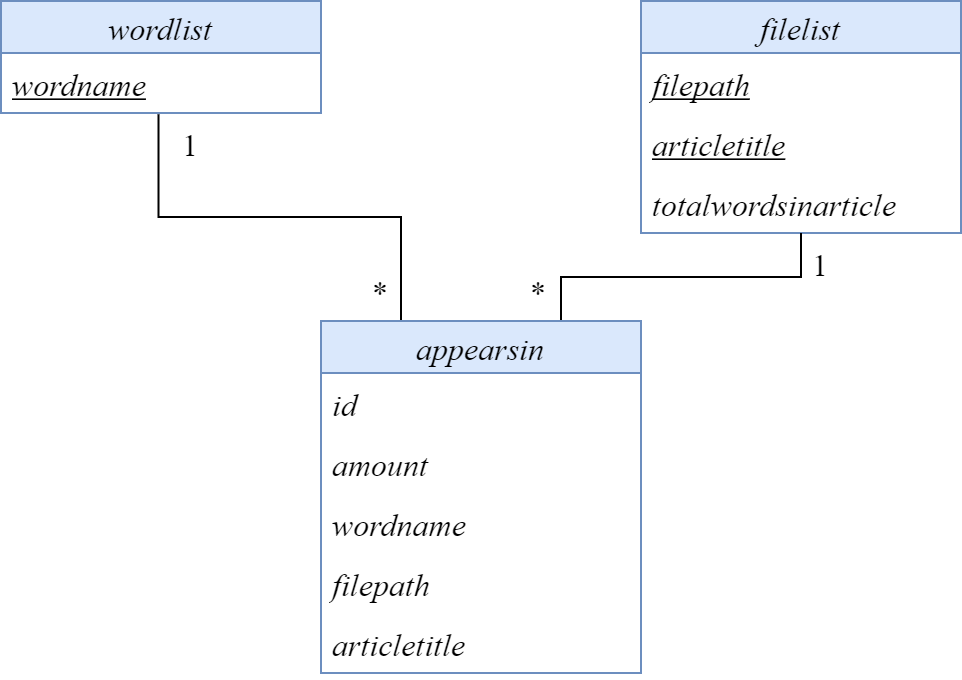
\includegraphics[width=\linewidth]{Images/old wordcount db.PNG}
    \caption{ER diagram of the relational database from last year.}
    \label{olddatabase}
\end{figure}